%!TEX TS-program = Arara
% arara: pdflatex: {shell: yes}
\documentclass[12pt,ngerman]{scrartcl}

\usepackage{babel}
\usepackage{xcolor}
\usepackage{tikz}
\usepackage{blindtext}

\begin{document}

\section*{TikZ und Nodes}

\blindtext

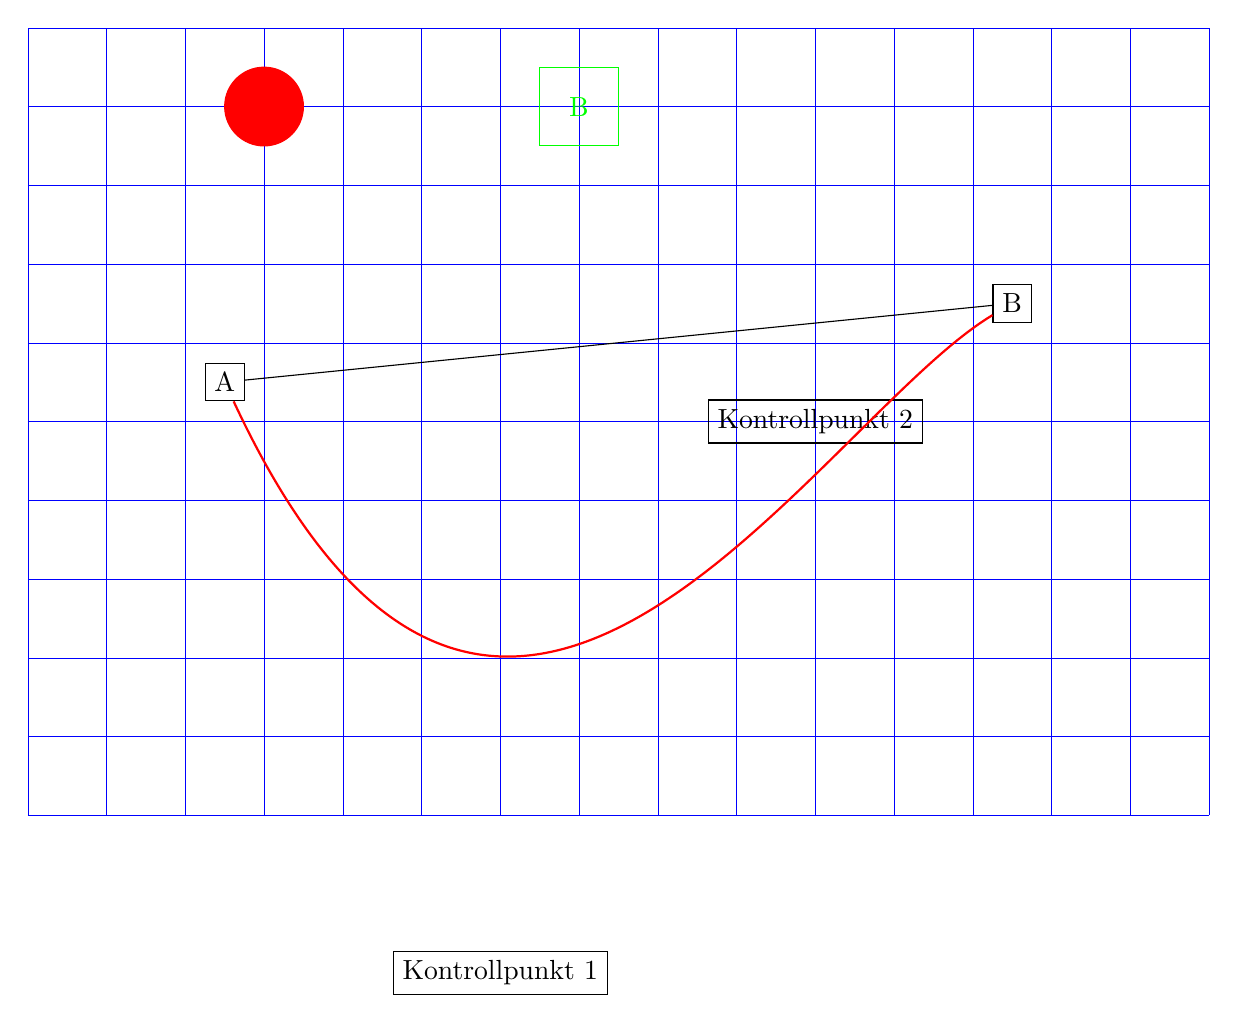
\begin{tikzpicture}
\draw[step=1cm,ultra thin,blue] (0,0) grid (15,10);

\node (c) at (6,-2)[draw]{Kontrollpunkt 1};
\node (d) at (10,5)[draw]{Kontrollpunkt 2};

\node (a) at (2.5,5.5)[draw]{A};

\node (b) at (12.5,6.5)[draw]{B};

\draw (a) -- (b);

\draw[red,thick] (a) .. controls (c) and (d) .. (b);

\node [draw,shape=circle,minimum size=1cm,fill,red] (e) at (3,9){};

\node [draw,shape=rectangle,minimum size=1cm,green] (f) at (7,9){B};


\end{tikzpicture}

\blindtext


\end{document}